%
% File acl2015.tex
%
% Contact: car@ir.hit.edu.cn, gdzhou@suda.edu.cn
%%
%% Based on the style files for ACL-2014, which were, in turn,
%% Based on the style files for ACL-2013, which were, in turn,
%% Based on the style files for ACL-2012, which were, in turn,
%% based on the style files for ACL-2011, which were, in turn,
%% based on the style files for ACL-2010, which were, in turn,
%% based on the style files for ACL-IJCNLP-2009, which were, in turn,
%% based on the style files for EACL-2009 and IJCNLP-2008...

%% Based on the style files for EACL 2006 by
%%e.agirre@ehu.es or Sergi.Balari@uab.es
%% and that of ACL 08 by Joakim Nivre and Noah Smith

\documentclass[11pt]{article}
\usepackage{acl2015}
\usepackage{times}
\usepackage{url}
\usepackage{latexsym}
\usepackage{graphicx}
\usepackage{caption}
\usepackage{amsmath}
\usepackage{hyperref}
\usepackage[numbers]{natbib}
%\setlength\titlebox{5cm}

\usepackage{listings}
\usepackage{xcolor}

\definecolor{codegreen}{rgb}{0,0.6,0}
\definecolor{codegray}{rgb}{0.5,0.5,0.5}
\definecolor{codepurple}{rgb}{0.58,0,0.82}
\definecolor{backcolour}{rgb}{0.95,0.95,0.92}

\lstdefinestyle{mystyle}{
    backgroundcolor=\color{backcolour},
    commentstyle=\color{codegreen},
    keywordstyle=\color{magenta},
    numberstyle=\tiny\color{codegray},
    stringstyle=\color{codepurple},
    basicstyle=\ttfamily\footnotesize,
    breakatwhitespace=false,
    breaklines=true,
    captionpos=b,
    keepspaces=true,
    numbers=left,
    numbersep=5pt,
    showspaces=false,
    showstringspaces=false,
    showtabs=false,
    tabsize=2
}

\lstset{style=mystyle}

% You can expand the titlebox if you need extra space
% to show all the authors. Please do not make the titlebox
% smaller than 5cm (the original size); we will check this
% in the camera-ready version and ask you to change it back.


\title{2024 COMP90043 Project}

\author{Author \\
Khai Fung Lee 1242579 \\
   \\\And
  Author \\
  Zhennan Zhu  1135920\\
  \\\And
  Author \\
  David Sha  1273615\\
  \\}

\date{25/6/2024}

\begin{document}
\maketitle
\begin{abstract}

\end{abstract}

\section{Background}
% 500 words
% Khai Fung
% Intro: Report outline (what will we be talking about)
% How does it work: X3DH & Double Ratchet Protocol
% Current word count: ~660 words
This project focuses on implementing and evaluating a robust key exchange protocol inspired by the Extended Triple Diffie-Hellman (X3DH) and Double Ratchet Protocol, which are core elements of modern secure messaging systems such as Signal Protocol. In this report, we will outline our implementation process and evaluate these protocols in great detail, including potential vulnerabilities in the protocol and analysis of its performance overhead in space \& time complexity.

\subsection{Motivation}
% Khai Fung
Let us preface by explaining how X3DH \& Double Ratchet protocol work. We will setup the scenario of Alice wanting to talk to Bob with Signal as an example. The first half of the Signal protocol is the X3DH, which aims to mutually authenticate Alice and Bob and then generate a shared secret key for secure communication.
\\
Initially, Bob sends a few public keys to the server: his identity public key $IPK_B$ (verifies identity of Bob), a signed public key $SPK_B$ (proves that he owns his identity private key and owns his one-time pre-keys), and a list of one-time session pre-keys $OPK_{B1}), OPK_{B2}, ...$ (to be used for each session of conversation with Alice).
\\
Since Alice wants to talk to Bob, the server will send her a pre-key bundle (Bob's identity public key $IPK_B$, his signed public key $SPK_B$, and one of his one-time pre-keys $OPK_B$) to help establish communication with Bob.
\\
Alice then generates her own identity public key $IPK_A$ and ephemeral key $EPK_A$ (a one-time use session key). With this, she will perform 4 Diffie-Hellmans (Figure \ref{fig:X3DH_1}) and append them together with a key derivation function (KDF) to produce the shared secret key that will be used to encrypt \& decrypt messages. She will then send a test message encrypted with this secret key and her public keys $IPK_A, EPK_A$ for Bob to recover the master key in the same way. The test message proves whether Bob is able to decrypt the message with the master DH key he created.
\\
\begin{figure}[htbp]
    \centering
    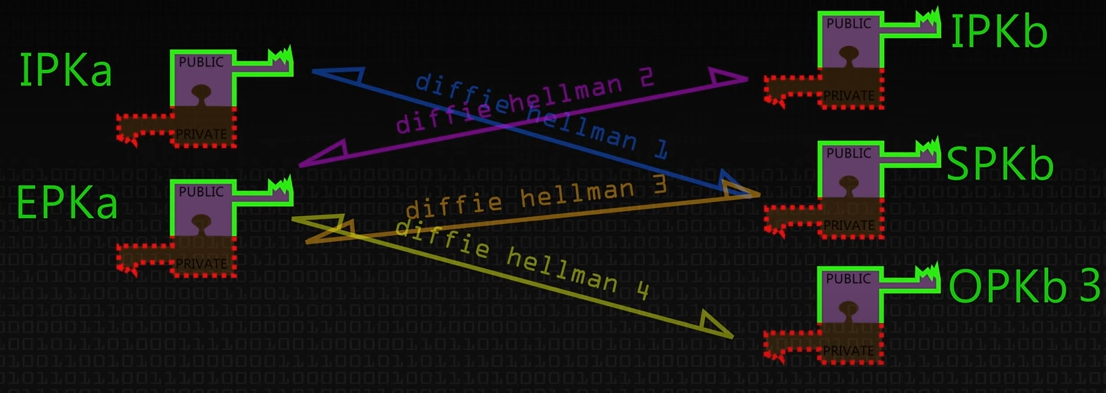
\includegraphics[width=1\linewidth]{images/X3DH 1.png}
    \caption{4 Diffie-Hellmans from Alice \& Bob's pre-key bundle}
    \label{fig:X3DH_1}
\end{figure}
\\
After X3DH is used to create a shared secret key, the Double Ratchet mechanisms are now used to facilitate the exchange of encrypted messages while dynamically updating the root key. The first 'ratchet' is a one-way KDF that Alice and Bob have a sending \& receiving ratchet of, used to derive new message keys from the chain key. The root key (obtained from X3DH) is passed through the KDF (with another input) to output a new chain key and new message key. So, for example in Figure \ref{fig:DR_1}, if Alice sends a message to Bob, she will use the KDF once to output a new message key $MK_{A1}$ to encrypt her message, which will lead to her sending ratchet ticking over. When Bob receives this message, his receiving ratchet will also tick over, in which he will pass through the same KDF with the same inputs to output the same message key $MK_{A1}$ to decrypt Alice's message.
\begin{figure}
    \centering
    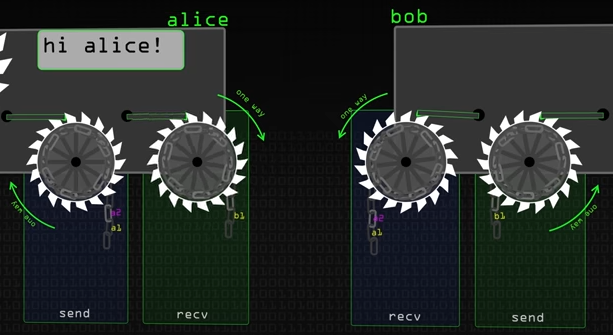
\includegraphics[width=1\linewidth]{images/image.png}
    \caption{Visual Diagram of Double Ratchet}
    \label{fig:DR_1}
\end{figure}
\\
This process is repeated for every message, where each message leads to Alice/Bob's sending/receiving ratchet ticking over and using the current chain key to output a new chain key and message key to encrypt messages [\ref{fig:DR_2}]. The one-way function ensures that previous messages won't be recovered if the current chain or message key is compromised.
\\
\begin{figure}
    \centering
    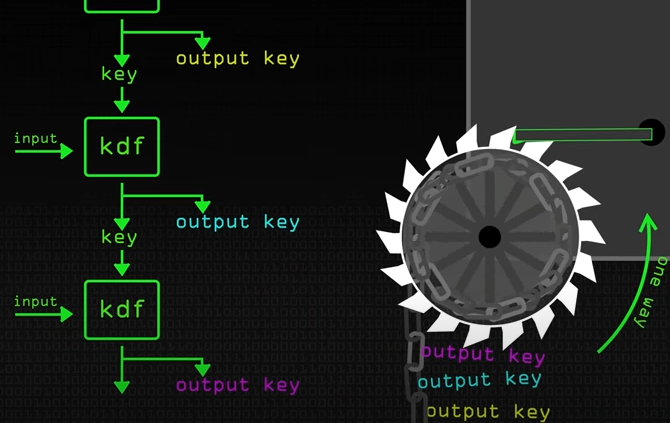
\includegraphics[width=1\linewidth]{images/DR_2.png}
    \caption{KDF Ratchet Function continuously running}
    \label{fig:DR_2}
\end{figure}
The second ratchet is a Diffie-Hellman ratchet that passes DH parameters as the other input into the KDF to ensure forward secrecy. These DH parameters can be used to 'reset' the first ratchet chain of message keys by creating a new master DH public key and thus update the root key.
\\\\
In the Evaluation section (Section \ref{eval}), we will analyze these two processes in more detail and justify the possible reasons why X3DH \& Double Ratchet protocol are a robust key exchange protocol.

\section{Implementation Process}
 % - 800 words

\subsection{Client and Server Architecture}
% David 200 words
We use a client and server architecture to model the real-world implementation of the Signal Protocol from Signal and other messaging applications alike. More specifically, the client and server architecture is modelled using Python classes (EXAMPLE) whereby we expose send (\texttt{Server.get\_bundle()}) and receive (\texttt{Server.recv()}) endpoints on the server that clients can use to perform its protocol operations. In our current implementation, the server specialises in sending and receiving data related to the X3DH protocol as indicated by the use of a \texttt{Server.get\_bundle()} function which is part of the second step in the X3DH protocol \cite{}.

\subsection{X3DH}
% David 300 words

\subsection{Double Ratchet}
Based on the Signal documentation, the Double Ratchet protocol is implemented using AES-based encryption and decryption functions. The following are some key functions of the implementation:

\begin{itemize}
    \item \textbf{RatchetInit(self, SK, bob\_dh\_public\_key)}: Initializes the user end.
    \item \textbf{KDF\_RK(self, rk, dh\_out)}: A key derivation function (KDF) to derive the chain key from the root key. \autoref{code:code_double_ratchet}

    \item \textbf{KDF\_CK(self, ck)}: A KDF to derive the message key from the chain key.
\end{itemize}

\begin{lstlisting}[caption={Sample Implementation of Key Functions}, label={code:code_double_ratchet}]
def KDF_RK(self, rk, dh_out):
    hkdf = HKDF(
        algorithm=hashes.SHA256(),
        length=64,
        salt=rk,
        info=b'info',
        backend=default_backend())
    derived_key = hkdf.derive(dh_out)
    receive_chain_key = derived_key[:32]
    send_chain_key = derived_key[32:]
    return receive_chain_key, send_chain_key
\end{lstlisting}


The following are key parameters chosen for the implementation:

\begin{itemize}
    \item \textbf{Curve: X25519}: An elliptic curve used to securely calculate the private and public keys.
    \item \textbf{Hash: SHA-256}: A cryptographic hash function used to generate a message authentication code (MAC).
    \item \textbf{Associated Data}: Some shared knowledge between users.
\end{itemize}

\textbf{Encryption} works as follows:
\begin{enumerate}
    \item Use \textbf{KDF\_CK} to derive a sending message key and create a header containing the new DH public keys, the message number of the previous chain, and the message number of the current chain.
    \item Create a random nonce from the HKDF-derive function using the key value as input, and encrypt the plaintext using the AES encryption algorithm.
    \item Generate an authentication tag (auth\_tag) as a message authentication code to ensure the integrity of the message.
\end{enumerate}

\textbf{Decryption} follows the same steps, with the additional check of the \texttt{auth\_tag} to verify message integrity before decryption.

% Andy

\section{Evaluation}\label{eval}
 % - 700 words

\subsection{Forward Secrecy and Cryptographic Deniability}
% Khai Fung
% Prove that forward secrecy & cryptographic deniability are satisfied... how?
% X3DH: satisfies cryptographic deniability due to the use of ephemeral keys (since the keys used by Alice won't be used in any following conversations with Bob), and since the shared secret key is created through DH, neither party can prove the key was generated by a specific individual, lack of digital signatures (but no non-repudiation results in lack of accountability when trying to verify messages, this is a natural flaw of end-to-end encrypted messaging apps like Signal and Whatsapp). Despite the lack of non-repudiation, Signal is still able to authenticate Alice & Bob's identity through safety numbers (outside of bounds of X3DH protocol).
% Double Ratchet: satisfies backward secrecy by the pre-image resistant nature of the KDF. If the current chain key is compromised, it will be hard to invert the KDF one-way ratchet to derive the previous chain and message key, thus making it difficult to decrypt past messages. Satisfies forward secrecy by the second DH ratchet deriving a new master shared key with new DH parameters every message. This means that attackers can't use old root keys with outdated DH parameters to derive new chain/message keys even if the KDF is public because Alice & Bob are frequently deriving new root keys.
X3DH satisfies cryptographic deniability for 3 reasons:
\begin{enumerate}
    \item Use of ephemeral keys: these are one-time use and won't be used in any following conversations with Bob
    \item Diffie-Hellman key generation: no one can prove the key was generated by any one individual
    \item Lack of digital signatures: can't prove who sent what
\end{enumerate}
However, cryptographic deniability means no non-repudiation, which results in a lack of accountability when verifying messages, which is a natural flaw of end-to-end encrypted messaging apps. Despite this, Signal can still authenticate Alice \& Bob's identity through safety numbers (Figure \ref{fig:safety-numbers}).
\begin{figure}[htbp]
    \centering
    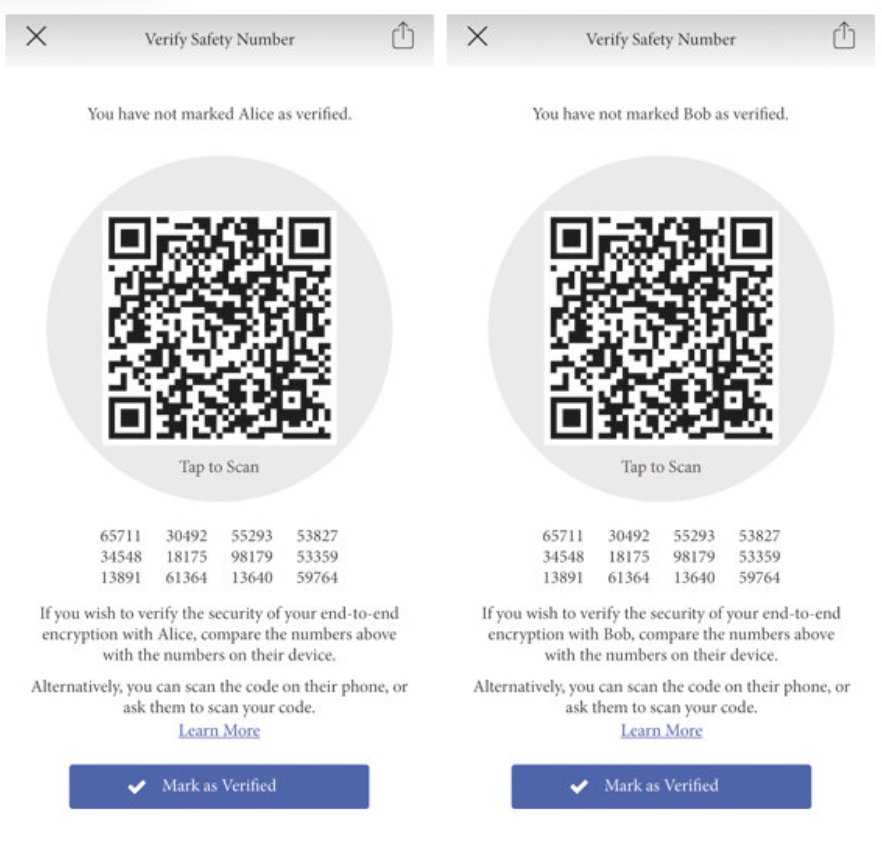
\includegraphics[width=1\linewidth]{images/safety_numbers.png}
    \caption{Identity authentication (done outside of the bounds of X3DH protocol)}
    \label{fig:safety-numbers}
\end{figure}

Double ratchet satisfies with the second DH ratchet deriving a new root key with new DH parameters every message. This means that attackers can't use old root keys with outdated DH parameters to derive new keys as new root keys are being created by Alice \& Bob each message.

% Why does Signal use X3DH & Double Ratchet over other alternative key exchange protocols?
% How can we manage keys more efficiently?
\subsection{Results Analysis}
If a user updates the Diffie-Hellman (DH) public key twice in a single message within the Double Ratchet algorithm, it could result in key synchronization issues between both parties, ultimately leading to communication failure.

% Everyone
\subsection{Performance Overhead}
% time and space complexity analysis

\subsection{Key Management and Lifecycle}
% Khai Fung
% Why do we use elliptic curve for key generation?
Signal Protocol employs elliptic curve for key generation, primarily due to its superior efficiency and security properties, compared to traditional cryptography methods like RSA. Compared to RSA, elliptic curve provides a higher level of security per bit (a 224-bit ECC key is equivalent to a 2048-bit key), thus making key sizes smaller but as secure \cite{mahto2017rsa}. This low computational overhead and memory is suitable for Signal as it is primarily used on mobile devices.

\subsection{Usability}
% how usable is the implemented code? How can it fit into other code for production use? Is it easy to integrate with other systems?


\subsection{Limitations of X3DH \& Double Ratchet}
% Khai Fung
% Potential weaknesses in Signal Protocol and possible improvement
%
Generally, we have found X3DH \& Double Ratchet to be one of the most robust key exchange protocol. However, we found that setting up and implementing the protocol from scratch was complex and hard to replicate.
\\
Furthermore, since Signal protocol relies on classical cryptography like ECC \& Diffie-Hellman, it could be broken by quantum attacks (). One way to future-proof against these attacks could be to integrate post-quantum algorithms such as Kyber into key generation. Duits (2019) pose various feasible post-quantum cryptography for Signal protocol.
\section{Conclusion}

\section{Appendix}

\subsection{Docker}
% Andy
% Implementation of the docker: 1. combination of protocols. 2. the client-server kind of interaction.

\bibliographystyle{plain}
\bibliography{refs}

\end{document}
